\chapter{Выборгское воззвание}

В субботу 8 июля 1906 года император Николай II подписал манифест о роспуске Государственной думы. Он не был до конца уверен в принятом решении, и, как гласит популярный в то время исторический анекдот, даже успел передумать в ночь на воскресенье. К окраинам столицы были стянуты войска, а в самом городе мобилизованы полицейские силы для подавления беспорядков.
Причины разгона Первой Думы кроются в самом её противоречивом разнообразии. Заменивший в апреле 1906 года С.Ю. Витте на посту премьер-министра Иван Логгинович Горемыкин не был готов идти на уступки депутатам, как это делал его предшественник. При Витте Дума позволяла себе поднимать в обсуждениях и выносить на голосование самые смелые проекты, касающиеся прав человека и земельных проблем. Новый глава правительства с порога заявил, что подобного своеволия больше не будет, за что был освистан. Депутаты требовали формирования ответственного перед Думой правительства и не собирались отступать.
В окружении императора нашлись министры, соглашавшиеся с “думцами”. Например П.А. Столыпин, назначенный в апреле на пост министра внутренних дел, активно вел переговоры с П.Н. Милюковым и С.А. Муромцевым о формировании кадетского правительства. Последние, чуя за собой силу, все меньше и меньше соглашались на уступки, отказываясь идти на компромисс. Подобный накал страстей не был случайным. Кадеты были уверены, что власть или пойдет им навстречу, или будет вынуждена столкнуться с всенародным протестом. Однако действующий премьер оказался более твердым, чем ожидалось. Именно по его инициативе Дума и была распущена монаршим повелением.

\begin{figure}[h!tb] 
	\centering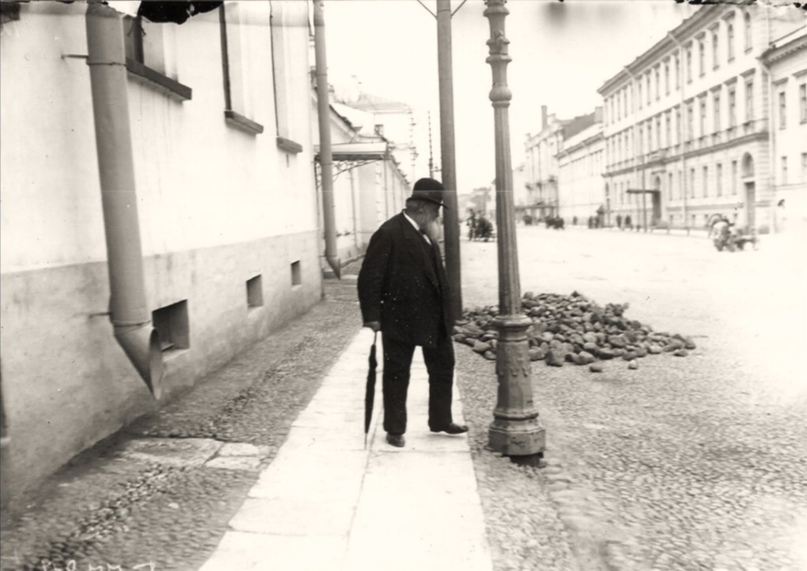
\includegraphics[scale=0.4]{Vozzvanie/JO61mEi5J00.jpg}
	%	\label{fig:scipion} % Unique label used for referencing the figure in-text\end{document}
	%	%\addcontentsline{toc}{figure}{Figure \ref{fig:placeholder}} % Uncomment to add the figure to the table of contents%----------------------------------------------------------------------------------------
	\caption{Депутат I Государственной думы идет на последнее заседание в Таврический дворец }%	CHAPTER 2
\end{figure}

\begin{figure}[h!tb] 
	\centering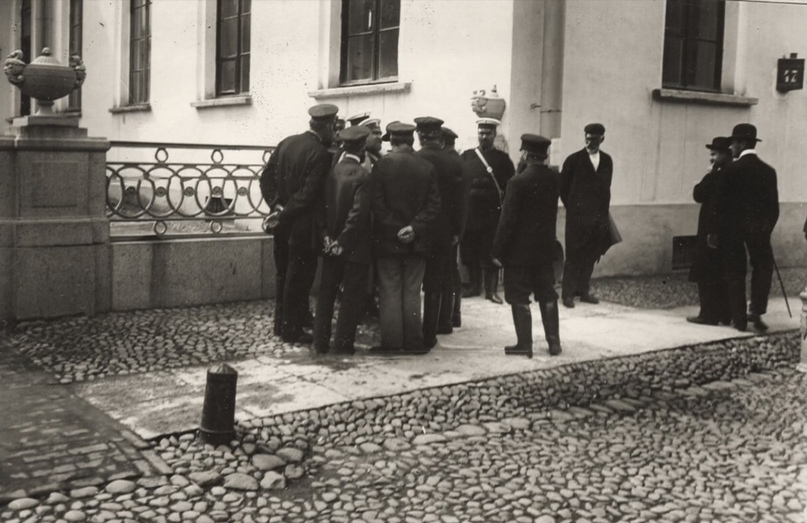
\includegraphics[scale=0.5]{Vozzvanie/aZhjQNDP7hY.jpg}
	%	\label{fig:scipion} % Unique label used for referencing the figure in-text\end{document}
	%	%\addcontentsline{toc}{figure}{Figure \ref{fig:placeholder}} % Uncomment to add the figure to the table of contents%----------------------------------------------------------------------------------------
	\caption{Депутаты I Государственной Думы возле Таврического дворца после роспуска Думы }%	CHAPTER 2
\end{figure}

Ожидаемых массовых волнений… не произошло. Столица и вся страна замерли в ожидании. На следующий день «Новое время» писало:
\begin{textcitation}
«Дума распущена... Город встретил это грустное известие спокойно. Все как будто растерялись от неожиданности и замерли. Думы больше нет, а к ней уже привыкли за эти два месяца».
\end{textcitation}

Близкое к кадетам и октябристам издание «Биржевые ведомости» еще в день подписания манифеста отмечало:
\begin{textcitation}
«Кажется, напрасно забили тревогу, совещались о порядке размещения войск по Петербургу на случай беспорядков и мобилизовали все полицейские силы. Ни для кого не тайна, что носилась мысль о роспуске Государственной Думы и о возникновении по этому поводу волнений».
\end{textcitation}
Да, депутатов не удивило такое развитие событий. Для большинства из них не было секретом, что власть, в конце концов, попытается сделать шаг назад в своих преобразованиях. Более того, многие политики ждали такого исхода, считая, что «Дума народного гнева» была лишь первой ступенькой в революции.
Самая активная часть образованной общественности видели в событиях 1905 года лишь прелюдию к более значимым переменам в жизни общества и государства. Перенося на Россию опыт европейских стран, многие политики считали эталоном Французскую революцию конца XVIII века. Они были уверены, что не может быть революции без своих Генеральных штатов и своего взятия Бастилии. И если Генеральные штаты в лице Думы уже появились, то им суждено быть как созванными, так и разогнанными. Значительная часть депутатского корпуса ждала разгона Думы, чтобы примерить на себя роль революционеров. Но вряд ли можно было ожидать «гильотин на площадях», как обещал в одной из бесед Столыпину Милюков — все же торжество Конституции было кадетам ближе, чем эпоха якобинцев.
Так курский депутат Василий Иванович Долженков говорил на заседании центрального комитета партии кадетов:
\begin{textcitation}
«Вот нас могут разогнать, и это будет замечательно! В Думу ворвутся солдаты со штыками. А я встану на мое кресло и скажу: «Мы скорее умрем, чем разойдемся!»
\end{textcitation}
Воспроизведение этих слов — такой же образец французской истории, как и депутатские ожидания. Долженков примерял на себя образ Оноре де Мирабо, который призвал коллег не расходиться по домам из зала для игры в мяч 20 июня 1789 года. Именно тогда Генеральные штаты превратились в Учредительное собрание, получив народную поддержку. Похожего эффекта желали и думцы, ожидая скорого, после роспуска Думы, социального взрыва.

\begin{figure}[h!tb] 
	\centering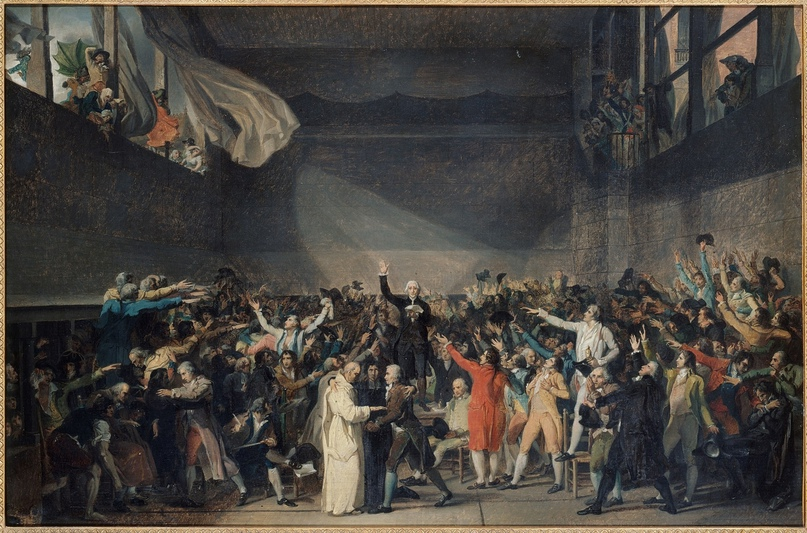
\includegraphics[scale=0.5]{Vozzvanie/85P4qo6DW7U.jpg}
	%	\label{fig:scipion} % Unique label used for referencing the figure in-text\end{document}
	%	%\addcontentsline{toc}{figure}{Figure \ref{fig:placeholder}} % Uncomment to add the figure to the table of contents%----------------------------------------------------------------------------------------
	\caption{именно так выглядит Русская революция}%	CHAPTER 2
\end{figure}

В России, однако, всё произошло гораздо более прозаично. Власть распустила Думу в выходной день, когда в Таврическом дворце было пусто и вставать на кресло с пафосными речами было некому. Стянутым к столице полкам не в кого было стрелять. Городовым некого было растаскивать. Часть депутатов на фоне этих событий решила обсудить дальнейший план действий, собравшись на квартире у одного из кадетов. Там обнаружилось, что наиболее активные члены партии — Иван Ильич Петрункевич и Фёдор Фёдорович Кокошкин уже придумали план дальнейших действий — депутатское воззвание к обществу.
Основная идея — пассивное сопротивление, как способ борьбы народа за свои конституционные права. Метод, на первый взгляд, неэффективный. В XX веке многие вспомнят лишь один успешный пример подобной стратегии — непротивление Махатмы Ганди. Однако члены партии Народной Свободы ориентировались на передовой, по их мнению, европейский опыт, а также на опыт уже произошедших в России событий.
Пассивное сопротивление предполагает вовлечение в протест широких масс обывателей, которые не склонны к политическому насилию. Им предлагается альтернатива, в которой они способны куда эффективнее проявить себя. Они могут открыто заявить о своем недовольстве властью и политической системой, отказавшись обеспечивать государство людскими и финансовыми ресурсами — не платить налоги и не идти в армию.

Так об этой технологии борьбы писал П.Н. Милюков:
\begin{textcitation}
«В промежутке между правительством и его органами с одной стороны и активными борющимися группировками с другой лежит обширная область общественных элементов более или менее пассивных. В острые политические моменты, подобные настоящему, от настроения этой средней, обыкновенно этой молчащей массы зависит необыкновенно много. Иногда от этого настроения зависит все, и стоит этому настроению выразиться, чтобы, как по волшебству, переменились декорации очередного момента».
\end{textcitation}
\begin{figure}[h!tb] 
	\centering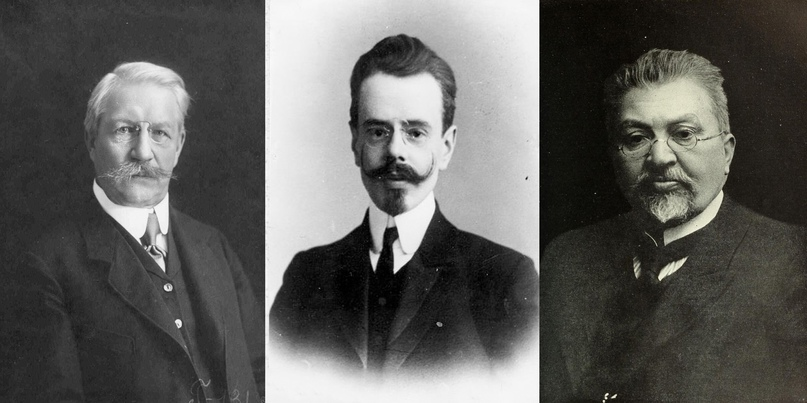
\includegraphics[scale=0.5]{Vozzvanie/jX4A4UFCctY.jpg}
	%	\label{fig:scipion} % Unique label used for referencing the figure in-text\end{document}
	%	%\addcontentsline{toc}{figure}{Figure \ref{fig:placeholder}} % Uncomment to add the figure to the table of contents%----------------------------------------------------------------------------------------
	\caption{Павел Николаевич Милюков, Федор Федорович Кокошкин-Младший и Иван Ильич Петрункевич
	}%	CHAPTER 2
\end{figure}

Данная тактика не была в новинку депутатам. Исторический опыт использования подобных методов борьбы можно было наблюдать во время Английской революции XVII века, в империи Габсбургов во время заключения соглашения 1867 года и в той же России незадолго до событий июля 1906 года.
Например, еще в октябре 1905 года Петербургский совет рабочих депутатов пытался дезорганизовать финансовую систему страны, призывая не платить налоги и забирать деньги из банков. Несмотря на то, что в депутаты совета были вскоре арестованы, такая тактика в полной мере оправдала себя. Мобилизация общественного мнения, активность городских дум и земств, формирование политических союзов, складывание партий, активизация прессы, забастовки— всё это, являясь, по сути, формой гражданского неповиновения без насилия, и подарило обществу Манифест 17 октября.
\textbf{Пассивное сопротивление — это «революция без революционеров»}. Это был призыв к обывателю. Наконец, победа пассивного сопротивления — это победа не силы, а организации. Организации не вооруженного восстания, на котором настаивали представители крайних партий, а организации общества, способного изменить ход истории. Так, по крайней мере, считали кадеты, подписавшие Выборгское воззвание.

И это были не просто депутаты, а самый сок кадетской партии. Ведущие ученые, социологи, юристы и правоведы, попытавшиеся спроецировать европейский опыт на Россию. Известные даже в Европе деятели, среди которых были Ф.Ф. Кокошкин, П.И. Новгородцев, Л.И. Петражицкий, В.Д. Набоков, С.А. Котляревский и другие, попытались осмыслить произошедшие в стране изменения и спланировать дальнейших ход событий.

\begin{figure}[h!tb] 
	\centering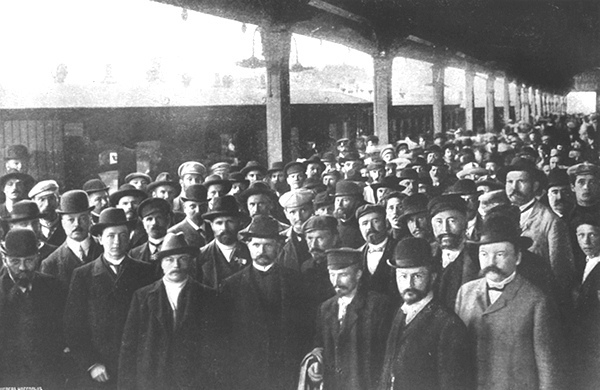
\includegraphics[scale=0.5]{Vozzvanie/C0fHlMQuvgM.jpg}
	%	\label{fig:scipion} % Unique label used for referencing the figure in-text\end{document}
	%	%\addcontentsline{toc}{figure}{Figure \ref{fig:placeholder}} % Uncomment to add the figure to the table of contents%----------------------------------------------------------------------------------------
	\caption{Депутаты Думы на Выборгском вокзале	}%	CHAPTER 2
\end{figure}

\begin{figure}[h!tb] 
	\centering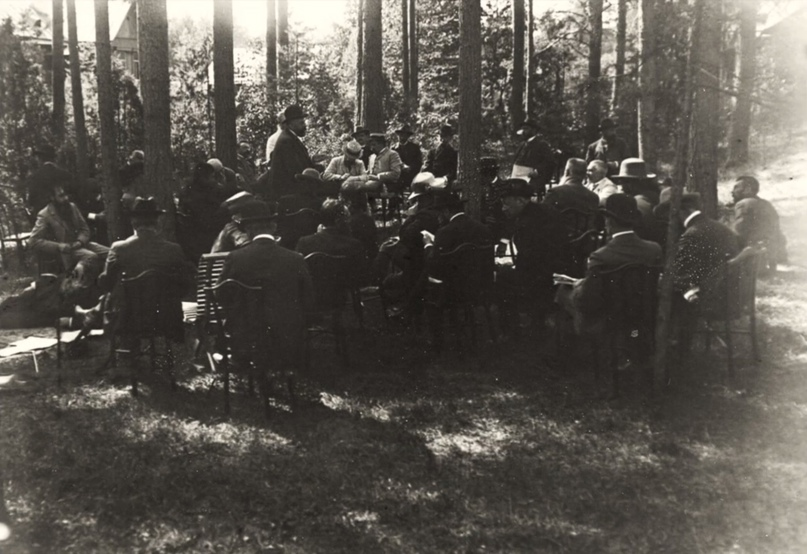
\includegraphics[scale=0.5]{Vozzvanie/heA6WdNPX0w.jpg}
	%	\label{fig:scipion} % Unique label used for referencing the figure in-text\end{document}
	%	%\addcontentsline{toc}{figure}{Figure \ref{fig:placeholder}} % Uncomment to add the figure to the table of contents%----------------------------------------------------------------------------------------
	\caption{Депутаты на собрании в Выборге	}%	CHAPTER 2
\end{figure}

\begin{figure}[h!tb] 
	\centering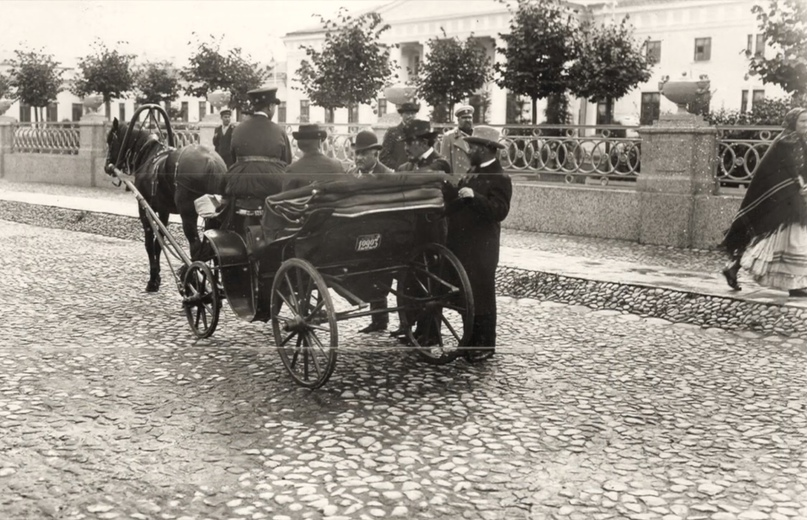
\includegraphics[scale=0.5]{Vozzvanie/xiieDslZycs.jpg}
	%	\label{fig:scipion} % Unique label used for referencing the figure in-text\end{document}
	%	%\addcontentsline{toc}{figure}{Figure \ref{fig:placeholder}} % Uncomment to add the figure to the table of contents%----------------------------------------------------------------------------------------
	\caption{Отъезд депутатов из Петербурга	}%	CHAPTER 2
\end{figure}
%Детали воззвания и его первый письменный вариант довел до совершенства глава партии Павел Николаевич Милюков. Тогда же, вечером 9 июля, было принято решение обсудить предполагаемое воззвание в Выборге, поскольку в Петербурге, как считали кадеты, уже распущенной Думе заседать не дадут. В город стали постепенно стекаться уже бывшие депутаты. Всего в тот день до Финляндии доехало около 180 человек, из них примерно 120 — кадеты. По воспоминанием многих думцев, место их официального собрания — гостиница «Бельведер» — не могла вместить всех желающих понаблюдать за историческим событием.
%В 16 часов 10 июля 1906 года воззвание было утверждено и подписано более чем сотней депутатов. Они провели почти всю ночь в бесконечных спорах о содержании текста, об опасностях, которые будут ждать их в столице, о смысле их протеста и будущем России. В течение следующего дня в Выборг приезжали опоздавшие. Некоторые доезжали специально с намерением поставить подпись. Другие, как тот же С.А. Котляревский, с намерением переубедить своих товарищей (кстати Котляревский в итоге воззвание подписал).

%Подлинник воззвания имел 170 подписей. Спустя некоторое время к нему просили присовокупить подписи еще 36 человек. Стандартный печатный вариант имел уже 181 подпись, часть из которых, как выяснилось позже, была поставлена или по доверенности от неявившихся депутатов или вовсе вместо них. Спустя несколько дней, недалеко от Петербурга прошла еще одна депутатская встреча, вошедшая в историю как Териокское собрание. На нем представители партии трудовиков предложили собрать исполнительный комитет разогнанной Государственной Думы, но, не получив поддержки кадетов, разъехались по домам.
\begin{figure}[h!tb] 
	\centering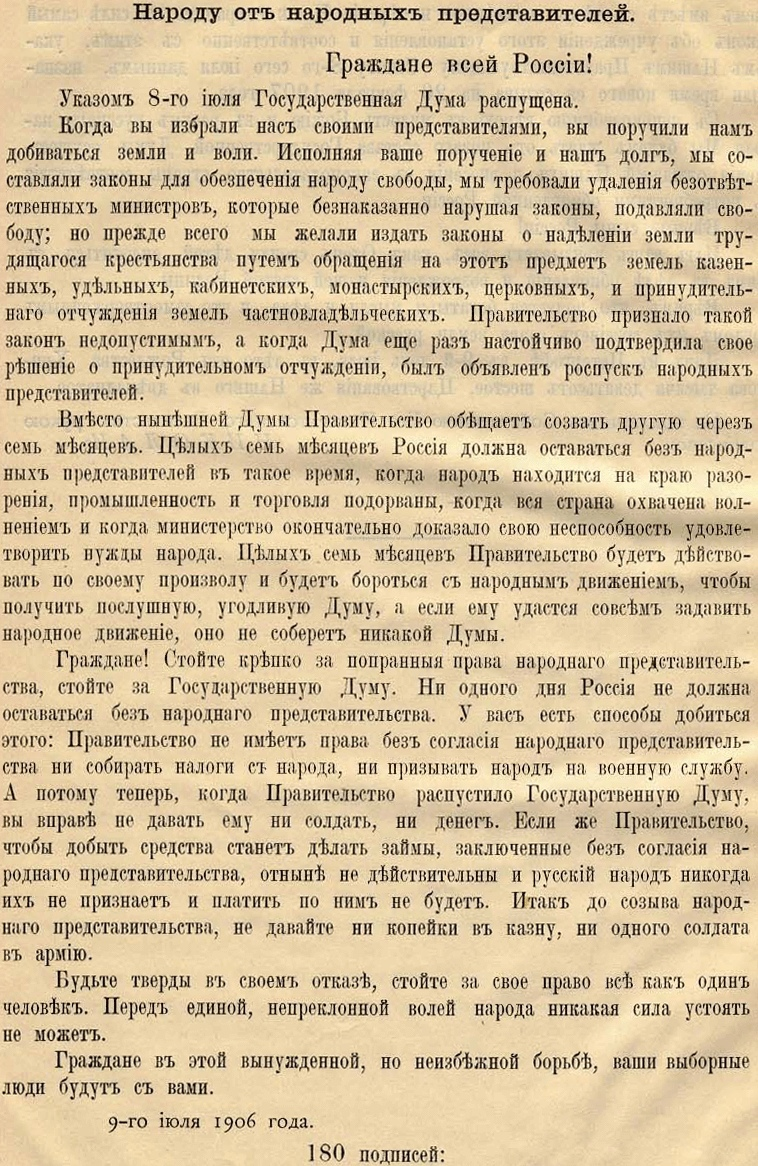
\includegraphics[scale=0.5]{Vozzvanie/MrEBj2VUCCs.jpg}
	%	\label{fig:scipion} % Unique label used for referencing the figure in-text\end{document}
	%	%\addcontentsline{toc}{figure}{Figure \ref{fig:placeholder}} % Uncomment to add the figure to the table of contents%----------------------------------------------------------------------------------------
	\caption{Фотокопия оригинального текста Выборгского воззвания}%	CHAPTER 2
\end{figure}

Отправившиеся же в из Выборга в Петербург депутаты воодушевленно пели «Марсельезу». Они ждали своего ареста и последующего народного гнева, который обрушится на власть. На Финляндском вокзале их встречало всего 200 человек, не считая жандармов. Большую часть толпы успели разогнать еще до приезда поезда. Всех приехавших посадили под арест, а потом начались уголовные дела…
Кажется, что никаких иных последствий, кроме ареста депутатов, подписавших воззвание, не было. Крестьяне продолжали все также нерегулярно платить прямые налоги. «Косить» от армии в 1906 году и вовсе стали меньше, чем в предыдущем. The end? Можно расходиться?
С одной стороны — да. Видимые последствия Выборгского воззвания минимальны. С другой — совсем наоборот.

В июле 1906 года власть чувствовала себя крайне неуверенно. Император вплоть до публикации манифеста не был уверен в своем решении о том, стоит распускать Думу или нет. Более того, роспуск Думы вовсе не означал её ликвидации. И во Второй Думе правительству придется столкнуться с не менее пестрым собранием депутатов, уровень доверия которых к власти будет еще ниже, чем у первопроходцев. Войска, подведенные к Петербургу и мобилизованные жандармы лучше всего говорят о том, что сам монарх и его окружение ждали взрыва социального недовольства. Его ждали и в Таврическом, и в Александровском дворцах. И там, и там считали, что революция только начинается.


\begin{figure}[h!tb] 
	\centering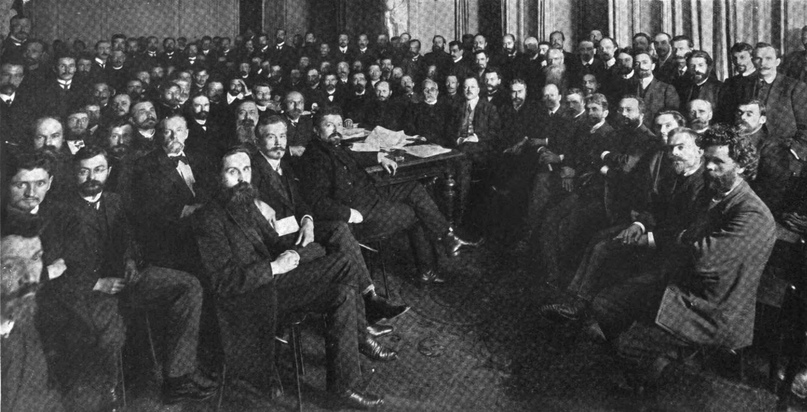
\includegraphics[scale=0.5]{Vozzvanie/qBWuVrrcLWg.jpg}
	%	\label{fig:scipion} % Unique label used for referencing the figure in-text\end{document}
	%	%\addcontentsline{toc}{figure}{Figure \ref{fig:placeholder}} % Uncomment to add the figure to the table of contents%----------------------------------------------------------------------------------------
	\caption{Объединённое заседание всех обвиняемых, бывших членов I Государственной думы по делу о «выборгском воззвании». 11 декабря 1907 г.
	}%	CHAPTER 2
\end{figure}

В июле 1906 года, как бы не утешала себя впоследствии власть, опасность стала слишком серьезной, чтобы её игнорировать. 26 октября 1906 года главноуправляющий имперской канцелярии Александр Андреевич Будберг говорил императору:

\begin{textcitation}
«…раз Россия проглотила роспуск Думы — вся либеральная Россия ничего не стоит, а раз она ничего не стоит, Ваше Величество, еще можете делать с нею делать что хотите».
\end{textcitation}

Однако вместо того, чтобы делать со страной «что хочется», власть еще в июне-июле 1906 года, медленно разворачивала те преобразования в социальной и экономической сферах, которые в будущем будут связаны с именем Петра Аркадьевича Столыпина.

Без ситуации июля 1906 года не было бы того курса, который ассоциируется с позитивными изменениями в жизни империи. Не было бы указа от 5 октября 1906 года об отмене ограничений в правах сельских обывателей, не было бы указа от 9 ноября, провозгласившего право крестьян на закрепление в собственность надельных земель, не было бы других преобразований правительства Столыпина.
Рассуждать об эффективности этих проектов сейчас, как и о всей ситуации июля 1906 года, довольно легко с позиции стороннего наблюдателя. Однако что созыв Думы, что её роспуск, что поворот правительства в сторону преобразований, воспринимались современниками тех событий как реальные вехи в развитии российской государственности и её политического строя. И, глядя на весь предшествующий опыт русской монархии, можно сказать, что они ими и были. И для подобных изменений не всегда нужна революция. Иногда достаточно лишь её ощущения.

\begin{figure}[h!tb] 
	\centering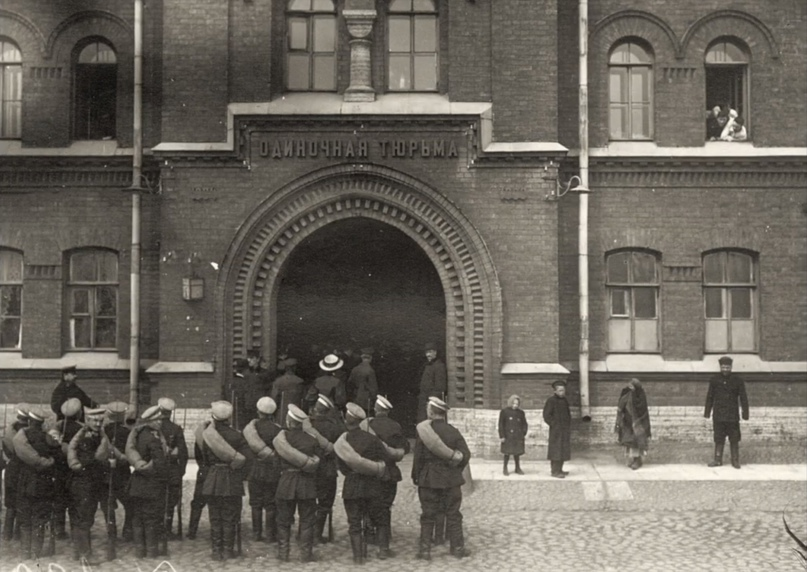
\includegraphics[scale=0.5]{Vozzvanie/isxQLVpDpX4.jpg}
	%	\label{fig:scipion} % Unique label used for referencing the figure in-text\end{document}
	%	%\addcontentsline{toc}{figure}{Figure \ref{fig:placeholder}} % Uncomment to add the figure to the table of contents%----------------------------------------------------------------------------------------
	\caption{Депутаты I Государственной думы, прибывшие отбывать трехмесячное заключение в Петербургской одиночной тюрьме (1)
	}%	CHAPTER 2
\end{figure}
\begin{figure}[h!tb] 
	\centering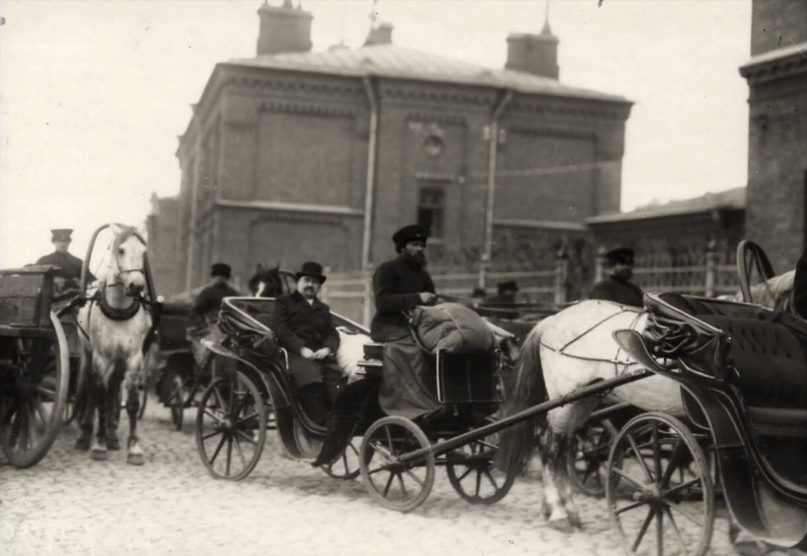
\includegraphics[scale=0.5]{Vozzvanie/cg8Te3zFzOQ.jpg}
	%	\label{fig:scipion} % Unique label used for referencing the figure in-text\end{document}
	%	%\addcontentsline{toc}{figure}{Figure \ref{fig:placeholder}} % Uncomment to add the figure to the table of contents%----------------------------------------------------------------------------------------
	\caption{Депутаты I Государственной думы, прибывшие отбывать трехмесячное заключение в Петербургской одиночной тюрьме (2)
	}%	CHAPTER 2
\end{figure}
\begin{figure}[h!tb] 
	\centering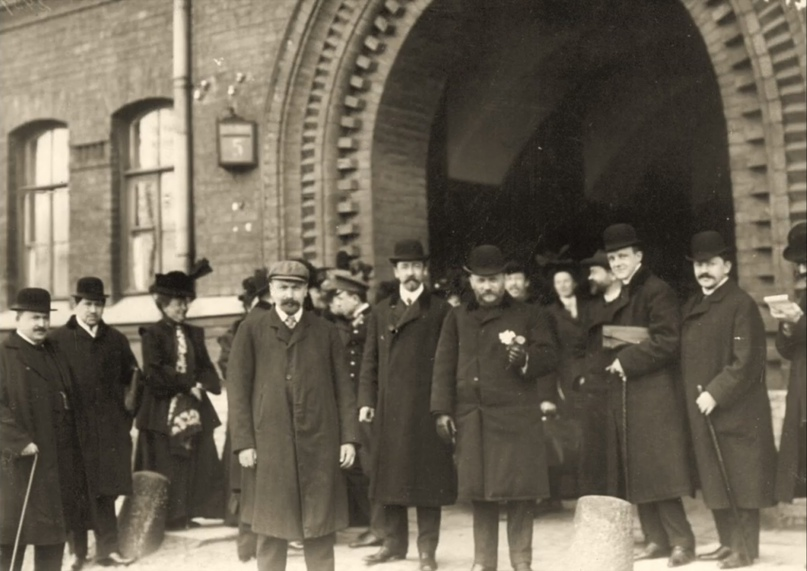
\includegraphics[scale=0.5]{Vozzvanie/ZOROnMVpx1c.jpg}
	%	\label{fig:scipion} % Unique label used for referencing the figure in-text\end{document}
	%	%\addcontentsline{toc}{figure}{Figure \ref{fig:placeholder}} % Uncomment to add the figure to the table of contents%----------------------------------------------------------------------------------------
	\caption{Депутаты I Государственной думы, прибывшие отбывать трехмесячное заключение в Петербургской одиночной тюрьме (3)
	}%	CHAPTER 2
\end{figure}
\begin{figure}[h!tb] 
	\centering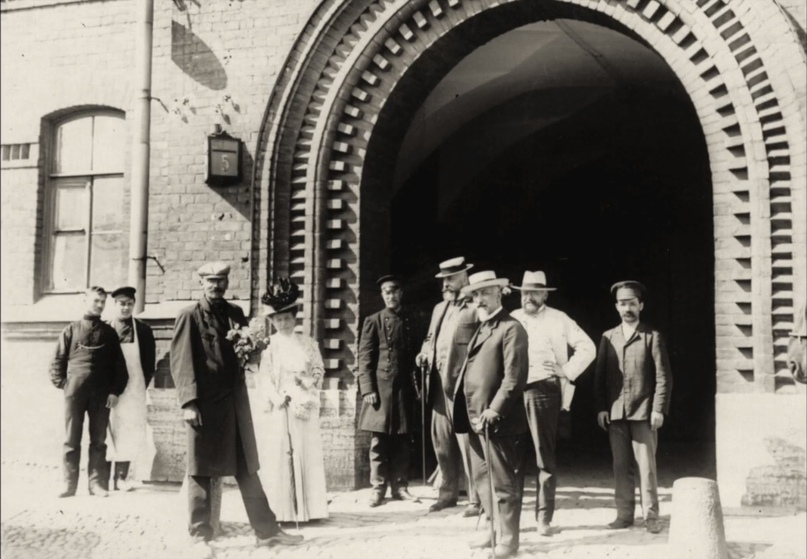
\includegraphics[scale=0.5]{Vozzvanie/VJ5dQO_XYFo.jpg}
	%	\label{fig:scipion} % Unique label used for referencing the figure in-text\end{document}
	%	%\addcontentsline{toc}{figure}{Figure \ref{fig:placeholder}} % Uncomment to add the figure to the table of contents%----------------------------------------------------------------------------------------
	\caption{Депутаты I Государственной думы, прибывшие отбывать трехмесячное заключение в Петербургской одиночной тюрьме (4)
	}%	CHAPTER 2
\end{figure}
\begin{figure}[h!tb] 
	\centering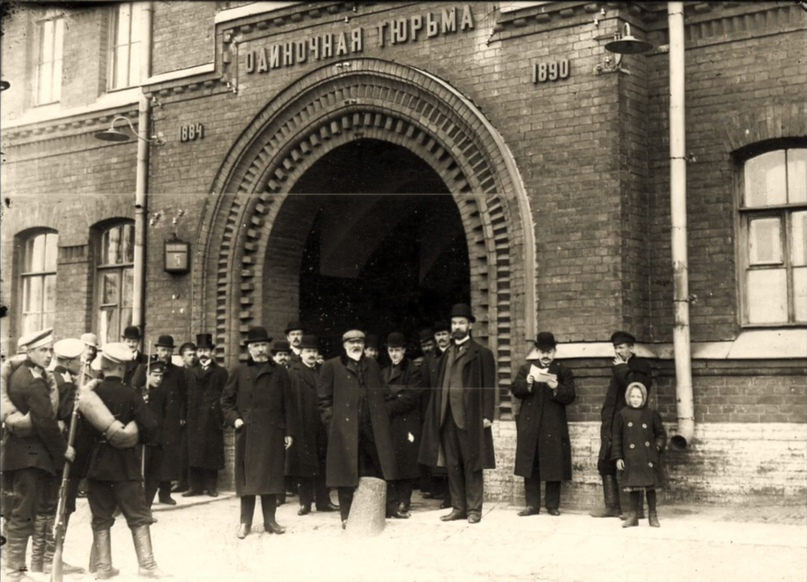
\includegraphics[scale=0.5]{Vozzvanie/vmMG0Vwk5sw.jpg}
	%	\label{fig:scipion} % Unique label used for referencing the figure in-text\end{document}
	%	%\addcontentsline{toc}{figure}{Figure \ref{fig:placeholder}} % Uncomment to add the figure to the table of contents%----------------------------------------------------------------------------------------
	\caption{Депутаты I Государственной думы, прибывшие отбывать трехмесячное заключение в Петербургской одиночной тюрьме (5)
	}%	CHAPTER 2
\end{figure}
\begin{figure}[h!tb] 
	\centering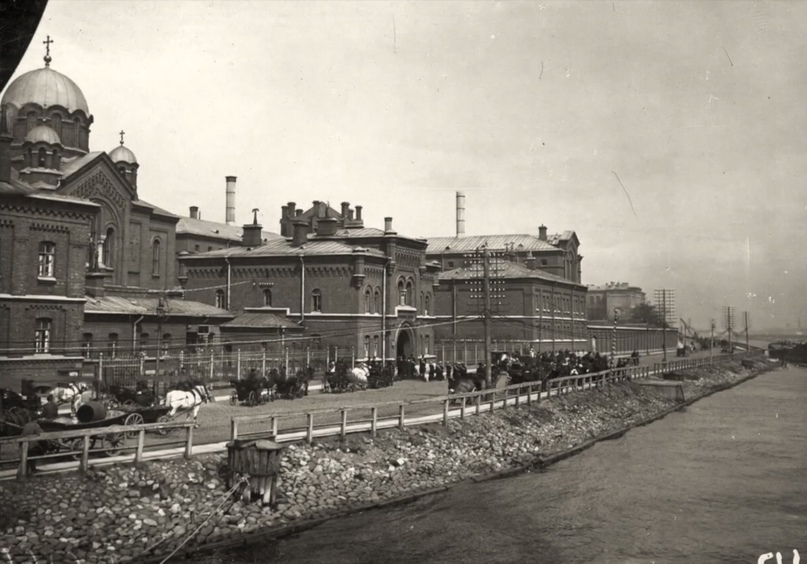
\includegraphics[scale=0.5]{Vozzvanie/xIJY3iaeRPA.jpg}
	%	\label{fig:scipion} % Unique label used for referencing the figure in-text\end{document}
	%	%\addcontentsline{toc}{figure}{Figure \ref{fig:placeholder}} % Uncomment to add the figure to the table of contents%----------------------------------------------------------------------------------------
	\caption{Депутаты I Государственной думы, прибывшие отбывать трехмесячное заключение в Петербургской одиночной тюрьме (6)
	}%	CHAPTER 2
\end{figure}

Большая часть депутатов, подписавших Выборгское соглашение, лишилась возможности вновь избираться в Государственную думу. Получив довольно мягкое, по меркам империи, наказание (они отсидели в тюрьме по три месяца), бывшие народные избранники не могли больше влиять на ход политической игры.
Однако для некоторых из них новый виток карьеры начнется уже после февраля 1917 года. Так Я.Я. Тыннисон станет первым премьером Эстонии, Н.Н. Жордания — председателем правительства демократической Грузии, Я.Х. Чаксте — президентом Латвии, а Ф.Ф. Кокошкин, М.М. Винавер и П.Н. Милюков, который хоть и не подписывал Воззвание, но повлиял на его создание, будут стоять у истоков Временного правительства.

Список использованной литературы:
\begin{enumerate}
	\item Галай Ю.Г. Основные законы Российской империи 1906 года и ограничение законодательных полномочий Государственной думы // Пробелы в российском законодательстве. 2009.
	\item Соловьев К.А. Политическая повседневность в 1906-1917 гг. М., 2019.
	\item Соловьев К.А. Выборгское воззвание: Теория пассивного сопротивления // Таврические чтения 2019. Актуальные проблемы парламентаризма: история и современность. СП-б., 2019
	\item Соловьев К.А. «Почему случаются революции?» // лекция в рамках проекта «Открытое пространство», 2019.
	\item Соловьев К.А. Выборгское воззвание: Теория и практика пассивного сопротивления. М., 2021.
\end{enumerate}

Автор Илья Агафонов Ссылка \url{https://vk.com/@com_pour_his-vyb-voz}
